\documentclass[LPSC_Labo03_SDeriaz]{subfiles}


\begin{document}
\section{Réalisation}
Tous les codes sont disponibles sur la page GitHub du projet\footnote{\url{https://github.com/SebastienDeriaz/LPSC_TP3}}
\subsection{Organisation}
Des fichiers "wrapper" sont utilisés pour gérer la connexion entre le bloc de calcul (loop ou pipeline) et l'interface de la BRAM. La structure du projet est décrite dans la figure \ref{fig_fichiers}

\begin{figure}[H]
\centering
\includegraphics[scale=1,page=4]{../Documents/Schemas-crop.pdf}
\caption{Organisation des fichiers}
\label{fig_fichiers}
\end{figure}
Les fichiers \verb!mandelbrot_loop.vhd! et \verb!mandelbrot_pipeline.vhd! se chargent de calculer une itération complète pour un pixel. Dans le cas du loop un pixel est réalisé à la fois, dans le cas du pipeline, les pixels sont envoyés à chaque coups d'horloge et les résultats sont présent après un délai de 100 coups d'horloge (le nombre maximal d'itérations).
\subsection{Itération}
L'itérateur (\verb!mandebrot_iteration.vhd!) est basé sur un process synchrone qui réalise tous les calculs en un coup d'horloge. Il est primordial d'avoir des registres sur toutes les sorties afin d'utiliser les itérateurs dans le pipeline ainsi que dans le loop.
\subsection{Loop}
Pour boucler, il suffit simplement de relier les sorties de l'oblitérateur sur les entrées (car elles sont équipées de registres). Lorsqu'un signal \verb!start! est actif, les entrées sont remplacées par des valeurs initiales.\\
Il existe aussi un process synchrone pour gérer les sorties du loop(\verb!done! et \verb!iterations!). Le process synchrone désactive la sortie \verb!done! lorsque le calcul est lancé et la ré-active lorsque le calcul est terminé, il va aussi mettre à jour la valeur de \verb!iterations!.
\subsection{Loop wrapper}
Le loop wrapper va utiliser le fichier \verb!ComplexValueGenerator.vhd! pour générer les nombres complexes et les transmettre au loop. Lorsqu'un pixel est calculé, le prochain est envoyé. Le loop wrapper est basé sur une machine d'état doit voici le graph
\begin{figure}[H]
\centering
\includegraphics[scale=1,page=5]{../Documents/Schemas-crop.pdf}
\caption{Machine d'état du loop wrapper}
\end{figure}
Le signal \verb!next_value! demande un nouveau nombre au générateur de nombre complexe (0 dans les autres états). Le signal \verb!loop_start! démarre le calcul du point (0 dans les autres cas).\\
La sortie du loop wrapper est une interface mémoire pour écrire dans la BRAM du \verb!lpsc_mandelbrot_firmware.vhd!
\subsection{Pipeline}
La base du pipeline est une boucle \verb!for generate! qui instancie 100 itérateurs. Le premier itérateur prend comme entrée les entrées du pipeline (point à calculer), le dernier itérateur fourni les sorties du pipeline (nombre d'itérations) et les itérateurs "centraux" sont reliés ensemble à l'aide de signaux. Afin de déterminer si la sortie du pipeline est valide (lorsque les données fournies à l'entrée sont arrivés à la sortie), le nombre d'itérations à la sortie doit être plus grand que 0 (car au moins une itération est toujours réalisée).\\
Les valeurs de \verb!Cr! et \verb!Ci! sont également propagées dans des registres pour fournir à chaque itération le bon point de départ. Ceci aurrait pu être réalisé dans les itérateurs pour simplifier un peu le code du pipeline.
\subsection{Pipeline wrapper}
Le pipeline wrapper est plus simple que le loop wrapper, il doit simplement transmettre les points fournis par le générateur de nombres complexes au pipeline à chaque coup d'horloge. Les valeurs à la sortie du pipeline sont directement écrites dans la BRAM du \verb!lpsc_mandelbrot_firmware.vhd!.\\
\subsubsection{Zoom}
Pour vérifier la vitesse de rafraichissement du pipeline, un zoom a été implémenté en faisant varier le point de départ et l'incrémentation du générateur de nombre complexe. Cette approche permet d'utiliser uniquement des compteurs et une incrémentation au lieu de stocker tous les zoom dans une mémoire (comme avec \verb!c_gen.vhd!).\\
Le zoom représente une grosse partie du process synchrone du pipeline wrapper mais consiste simplement en un compteur qui fourni une horloge à \SI{10}{\hertz} pour effectuer l'itération de zoom et un autre compteur pour revenir à l'état initial (pas de zoom) après une centaine. Il y a aussi un temps d'attente de $\approx$\SI{1}{\minute} dans l'état de zoom minimal et maximal afin de laisser le temps d'observer la fractale.
\subsection{Résolution des couleurs}
Afin d'obtenir une meilleure résolution de couleurs, le nombre d'itérations a été stocké dans la mémoire (au lieu de la couleur de chaque pixel) et la LUT est appliquée à la sortie de la mémoire (côté HDMI), ceci permet de diminuer le nombre de BRAM utilisés (7 bits stockés au lieu de 9) tout en améliorant la fidélité des couleurs.
\subsection{Fréquence}
Avec l'implémentation du pipeline, il existait un "worst negative slack" de \SI{-8}{\nano\second} avec une fréquence de \SI{100}{\mega\hertz}. Comme le pipeline est capable de générer l'image à raison de 1 pixel par coup d'horloge, ceci donne un framerate de environ 163 images par seconde ce qui est inutilement important. La fréquence a donc été diminuée à \SI{50}{\mega\hertz} pour respecter les contraintes de timing tout en ayant une fréquence de rafraichissement largement confortable de 81 images par seconde.







\end{document}